\chapter{Word Embeddings}\label{ch_word_embeddings}
\chapterauthor{Ellis Cain, Jeff Yoshimi}

% Also see online doc NLP Exercises
% TODO: Go through chapter and add glossary items
% Cohere tokens concept with transformer chapter

This chapter elaborates on the concept of a word embedding, which was briefly discussed in section \extref{wrangling}. A word embedding associates words and word parts (tokens) with vectors in a way that that captures important characteristics of those tokens. In this way tokens can be ``embedded'' in a vector space, that is, associated with lists of numbers that can in turn be processed by a neural network, and associated with points in a space. These techniques have a long history in linguistics and in the study of neural networks, but have become especially prominent in recent years with the advent of large language models like GPT (section \extref{transformers}). Given the emphasis on converting words and other linguistic entities to vectors, this chapter also sheds further light on the concept of feature engineering (section \extref{wrangling}) and ``wrangling'' data so it can be used in neural networks.

After giving some background on linguistics and natural language processing, we build up to the concept of a word embedding in stages. First we discuss document embeddings (associating whole documents with vectors of numbers), which are simpler to understand and serve as a useful basis for understanding word embeddings.  Then we discuss word embeddings. Then we discuss the kind of pre-processing and workflow often involved in actually taking a text, creating an embedding, and feeding it to a statistical model like a neural network. Finally we give a brief summary of ways neural networks are used to process linguistic data that has been numerically coded with a text embedding.\footnote{Formally a word embedding is a function from a set of tokens to a set of vectors, and a document embedding is a function from a set of documents to a set of vectors.  We will use ``text embedding'' as a generic way to cover both cases.}

\section{Background and History}

Linguistics is the study of language, which can be organized in terms of scale, going from smallest to largest unit of study: 
\begin{enumerate}
\item Phonetics and phonology: the study of speech sounds.
\item Morphology: the study of words and word forms.
\item Syntax: the study of the structure or grammar, usually at the sentence level.
\item Semantics as the study of meaning, which can be at a variety of levels (words, phrases, sentences).
\item Pragmatics as the study of intentional meaning or implied meaning, for exams implicit maxims and rules of conversations (Grice). 
\end{enumerate}

% Clearly more is needed here, and the above needs to be cleaned up (e.g. the stray Grice citation).  A bit of fleshing out and more citations.
Researchers often use spectrograms to analyze phonemes (the smallest units of sound, e.g. /t/ or /p/). As you increase the scope of analysis it increasingly becomes more difficult to (automatically) analyze linguistic data. For syntax, there are treebanks and dependency analyzers that have to be trained on lots of example hand-annotated data to be able to analyze new sentences. There are also reasonable limits per word (for syntactic analysis), a word usually has one or two parts of speech (noun, verb, determiner, etc.), and there are constructed rules for how to derive dependency trees. What about meaning for semantics? There isn't a clear unit of ``meaning'' for words: meaning is more broad and nebulous. The meaning of a word can be abstract or concrete (``justice'' vs ``cup'') and is often context dependent (``bass'' as the fish or instrument). How could we automate the analysis of semantic information?

% A bit more needed on comp ling in general.
Of course the history of linguistics is complex, but in the context of neural networks one particular strand, computational linguistics, is especially important. 

%WordNet is a lexical database of English constructed by linguists, where words are organized into ``synsets'' (cognitive synonyms or groups of words). Similarity is calculated using the Wu-Palmer path similarity function which is based on the number of jumps between synsets.

%% Commenting this out until structure of chapter is more clear
%\subsection{Early text embeddings}
%
%% TODO: Check and fix
%One early approach was to simply manually create feature vectors based on linguistic attributes.  For example, in Elman's ``Finding structure in time''~\cite{elman1990finding}, each of 6 words was associated with a 31-bit vector.  Some examples are shown in figure \ref{elmanWordEmbeddings}.
%
%\begin{figure}[h]
%\centering
%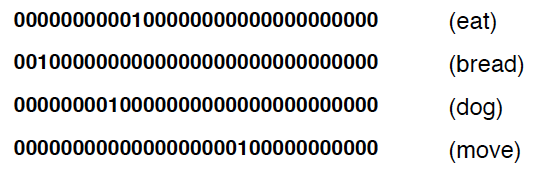
\includegraphics[scale=.5]{./images/elmanWordEmbeddings.png}
%\caption[From \cite{elman1990finding}.]{Some of Elman's word embeddings. }
%\label{elmanWordEmbeddings}
%\end{figure}
%
%These early embeddings were hand-crafted based on the scientist's intuitions or using other simple techniques to ensure certain similarity structures. Besides these hand-crafted methods, automated forms of meaning analysis were developed. These automated approaches take documents and use the information in them to produce ``text'' embeddings.
%

\section{Document embeddings}

% Some history on this and why it was done would help. Why do people do this? How is this useful? 
One simple idea in the background of many text embeddings is the \glossary{bag of words} approach, which associates documents with vectors of word frequencies. This approach ignores grammatical structure and just looks at how often different tokens occur in different documents.  Simply put, we take each document and put the associated tokens into a bag, and count up how many tokens occur in each bag. Consider the following documents

\begin{description}
\item[Document 1]  ``The bass fish played the bass''
\item[Document 2]  ``The fish played fish with the fish monger''
\end{description}

Each document will be associated with a bag of words, as shown in figure \ref{exampleBags}.

\begin{table}[h]
    \centering
    \begin{tabular}{|l|c|c|c|c|c|c|}
    \hline
    Bag of words & the & bass & fish & played & with & monger \\
    \hline
    Document 1 & 2 & 2 & 1 & 1 & 0 & 0 \\
    Document 2 & 2 & 0 & 3 & 1 & 1 & 1 \\
    \hline
    \end{tabular}
    \caption{Bag of words representation}
    \label{exampleBags}
\end{table}
These document-level bag of words embeddings have a number of problems. First, they ignore the syntactic structure of the sentences in the documents they encode.  Second, they are influenced by the uneven distribution of certain terms in natural languages \cite{piantadosi2014zipf, zipf1945meaning}. To counteract this, we can use TF-IDF (term frequency-inverse document frequency) to calculate the importance of a specific term for a (set of) related document(s), which offsets how frequently a term appears (term frequency) by the number of other documents that also contain the term. This allows it to focus on meaningful terms and not those that generally appear frequently (`the', `a', etc.). 
% Only defined for sets of documents. Places higher weight on terms that occur frequently in one document but not in others. Terms that occur frequently in all documents are given less weight (the inverse document frequency).  Does not address syntax but does deal with distribution issue. Used originally for information retrieval.  This admubrates PPMI in word embeddings.

LSA (latent semantic analysis) is used with a set of documents to analyze semantic information and calculate document similarity. The set of documents is represented using a document-term matrix, where each row corresponds to a document, and each column corresponds to the frequency of a given term (see table \ref{exampleBags}). Then, singular value decomposition (SVD) is used for dimensionality reduction (see \extref{S:dimred}), resulting in a numeric vector for each document (based on term usage/frequency) which can be compared using cosine similarity (section \extref{dotProduct}) to get document similarity.
% So basically SVD on bag of words

% Maybe add some examples
These methods are calculated at the document level: calculating term frequencies in a given document or set of documents. We can then use these document embeddings to to calculate document similarity, as with LSA.
As we will see in the next section, these methods can also be adjusted and applied to the word level as well, allowing us to quantify word meaning as word embeddings. That is, the methods of document embeddings can be used to come up with word embedding techniques, and these word embeddings can be used to calculate how similar words are to each other.

\section{Word embeddings}

We now move from document embeddings to word embeddings.  Instead of associating documents with vectors, we associate words with vectors. To begin to get a feel what word embeddings are before we discuss the details, see \url{http://vectors.nlpl.eu/explore/embeddings/en/}. Word embeddings are very important in neural networks and machine learning. A well-known example is Word2Vec \cite{mikolov2013distributed} which tracks the linguistic context and word co-occurrences to ``embed'' words into a semantic space.\footnote{A code-based walk through of the algorithm is here:  \url{https://www.tensorflow.org/tutorials/word2vec}.} The general idea is that the generated embedding space is much like our own semantic space \cite{lewis2019distributional}, with the advantage that we can track and compare word meanings mathematically and visually, as in figure \ref{f:writerPainterExample}. 

\begin{figure}[h]
    \centering
    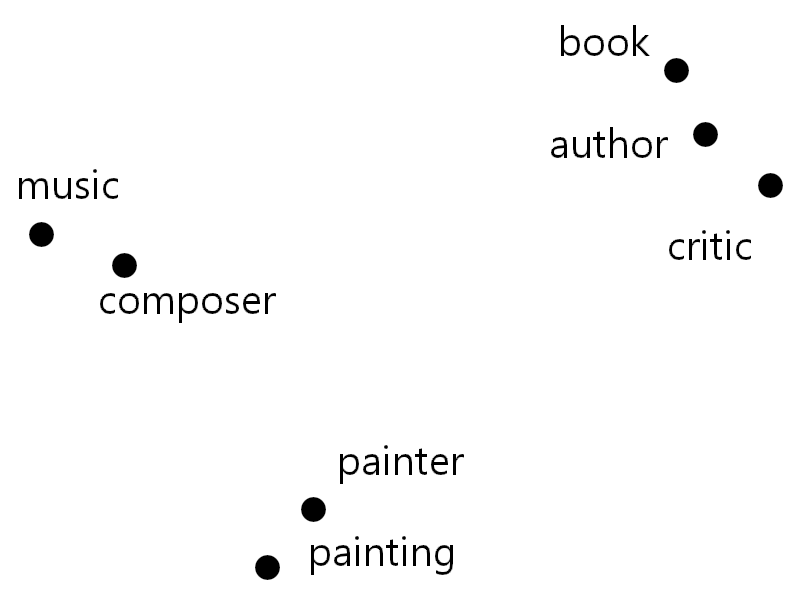
\includegraphics[scale=.5]{./images/Word_vector_demo.png}
    \caption[Generated using \url{http://vectors.nlpl.eu/explore/embeddings/en/}.]{Example of word embeddings in a semantic space. An embedding space for the seven words: ``book'', ``author'', ``critic'', ``music'', ``composer'', ``painter'', ``painting''. The embeddings demonstrate how the creator of a medium would be close to the medium or composition. Interestingly, ``critic'' is closest to ``author'', perhaps due to most critics \textit{writing} their criticism.}
 \label{f:writerPainterExample}
\end{figure}

 
\subsection{Distributional Semantics Theory}

Theoretical support for this method of computing word embeddings (i.e., tracking co-occurrences allows for a rough estimation of word meaning relative to other words) is provided by the theory of distributional semantics \cite{harris1954distributional, firth1957synopsis} and other usage-based theories of language \cite{wittgenstein1953philosophical}, which posit that the usage of words reflects their meaning, and information about the meaning of words is embedded in linguistic context and the statistical properties of language usage.

This is often illustrated with the following quote, attributed to John Firth: ``You shall know a word by the company it keeps.'' For example, when someone talks about a \textit{river}, they may also mention \textit{water} or \textit{bank} (as in river bank), helping the listener correctly decode the intended meaning. Or, from the quote, you are able to interpret \textit{company} as referring to other words in the sentence, and not a \textit{business}, based on the earlier context.

By connecting usage to meaning, this allows for an approximation or representation of meaning that is derived from usage in a text corpora. Instead of analyzing large corpora by hand, computational algorithms can be used to generate numeric representations.

\subsection{Word Embeddings and Co-occurrence Matrices}

% Todo: no single quotes. Glossary or ital instead? Also a problem is that target and label have other meanings in the book.  In 
% Jeff can do a pass just expanding this a bit, defining each part, maybe with some pictures. How do they work on edges? Or we can work on it  together. One specific question that comes up below is what to do with windows, do they scan across sentences?

%% skip-gram is similar to masked token prediction -- using the bi-directional context, predict the masked target.
Broadly speaking, to construct a co-occurrence matrix, we must iterate across every sentence in the document or training corpora, where we iterate across each word and count the co-occurrences with the surrounding context. Each word is iterated as the `label' or `target', while the surrounding words serve as the `context'. A window size is defined, which designates how many words to include in the `context'. This context can be either unidirectional, using the preceding text, or bidirectional, using all surrounding context. Once the whole training corpora has been processed, the result is a co-occurrence matrix where each cell represents the raw co-occurrence counts for a given label-context pair.

% Also good but needs to be broken out a bit more into parts and definitions.  In particular for PPMI
Not every word is used with the same frequency. Similar to our document embeddings, some determiners (`the', `a') may be over-represented and skew the co-occurrence matrix. If these type of \emph{stopwords} were not removed, we can change the weight of different contexts. Therefore, a positive-pointwise mutual information (PPMI) transform is often used to weight the matrix. Lenci~\cite{lenci2018distributional} explains PPMI as measuring ``how much the probability of a target-context pair estimated in the training corpus is higher than the probability we should expect if the target and the context occurred independently of one another.''

In other words, PPMI weights the co-occurrence values to avoid word-frequency-bias in embeddings. Words like ``the'' and ``a'' that should not be considered meaningful in terms of co-occurrence are down-weighted. Less frequent words on the other, like ``platitude'' or ``espresso'', that are more meaningful in terms of co-occurrences, are up-weighted. The result is a set of \textit{n}-dimensional vectors for a set of words, which are referred to as ``word embeddings.'' For a more in-depth explanation and discussion of word embeddings and distributional semantics, see \cite{lenci2018distributional}.

% \textbf{Quote from Lenci:} PPMI measures how much the probability of a target-context pair estimated in the training corpus is higher than the probability we should expect if the target and the context occurred independently of one another. (Lenci, 2018)

\subsection{Evaluation of word embeddings}

How should these embeddings be evaluated? Previous research on word similarity and relatedness has shown that directly asking for relatedness judgements can accurately capture word relations \cite{finkelstein2001placing}.

Therefore, the general method of evaluation is by collecting a set of human judgements, which theoretically serve as the ceiling of model of model performance, though there are recent discussions questioning this \cite{richie2022inter}.
There are a variety of gold standards that have been used across the field, such as WordSim-353 \cite{finkelstein2001placing, agirre2009study}, however, recent models have already reached or surpassed human performance on these tasks.

% Ellis we should discuss this and unpack
Since the models had reached the theoretical performance ceiling based on the gold standards, it was problematic for the field; how would future changes or improvements be evaluated if performance was already at the max?
In response to this, Felix Hill and colleagues \cite{hill2015simlex} set out to create a gold standard that separates similarity from association (previous standards had ignored the distinction) and therefore create a better gold standard that points the way forward for development. 

In brief, association and similarity are two different concepts. Association refers to a relatedness between two concepts, whereas similarity refers almost to synonymy. A major point in their paper \cite{hill2015simlex} is that these two concepts can be separated.
For example, ``car'' and ``tire'' would be considered associated but not similar, while ``glasses'' and ``spectacles'' would be similar.
Interested individuals can read the paper for a more in-depth discussion and model comparison. This issue has become less prominent with the advent of BERT and LLMs.

While different algorithms may improve the model performance and similarity to our own semantic representations, the corpus quality also has an impact on model performance.
Larger training corpora generally improve the quality of the derived embeddings, since the increased amount of data ideally adds more context to be processed. 
GloVe embeddings are trained on various training corpora, varying from 1 billion tokens to 42 billion tokens \cite{pennington2014glove}.

Beside the amount or size of the training corpora, the type of documents is also important; training solely on works of fiction would lead to different embeddings than a model trained on non-fiction, and so on. It is important to consider the meaning you are trying to capture (generalized or specific to a field, such as medical documents).

\section{Workflow}

Now to get our hands dirty. In practice there are many steps involved in applying these ideas. 
Here is a sample workflow or pipeline:
\begin{enumerate}
\item Sentence segmentation.
\item Word tokenization
\item Normalization and filtering
\item Creation of word embeddings
\end{enumerate}

To get a sense for how this works, let's apply this pipelines to a sample document:

\begin{quote}
My work is a matter of fundamental sounds, made as fully as possible. Even though they are fundamental, they bring rich aromatic hints of humor. If people want to have headaches among the overtones, let them. And provide their own aspirin. (Adapted from a letter from Samuel Beckett to Alan Schneider, 1957)
\end{quote}

Sentence segmentation.  For sentence segmentation, the paragraph or document is segmented into sentences. This step is particularly important when using text that has been scanned using OCR, where errors might occur. Our sample document would be segmented into three sentences (given that we are segmenting just on periods):

\begin{enumerate}
    \item \textit{My work is a matter of fundamental sounds, made as fully as possible.}
    \item \textit{Even though they are fundamental, they bring rich aromatic hints of humor.}
    \item \textit{If people want to have headaches among the overtones, let them.}
    \item \textit{And provide their own aspirin.}
\end{enumerate}

Word tokenization. Once the document has been segmented into sentences, a tokenizer is used to split each sentence into the comprising words. This yields a list of lists of tokens, as in
\begin{enumerate}
    \item \textit{my, work, is, a, matter, of, fundamental, sounds, made, as, fully, as, possible}
    \item \textit{even, though, they, are, fundamental, they, bring, rich, aromatic, hints, of, humor}
    \item \textit{if, people, want, to, have, headaches, among, the, overtones, let, them}
    \item \textit{and, provide, their, own, aspirin}
\end{enumerate}

Normalization. Following tokenization, the words/tokens are generally normalized to remove capitalization or certain punctuation marks, such that the words are consistently in the same form. In this step, stopwords can be filtered out. In our case:
\begin{enumerate}
    \item \textit{work, matter, fundamental, sounds}
    \item \textit{fundamental, bring, rich, aromatic, hints, humor}
    \item \textit{people, headaches, overtones}
    \item \textit{provide, aspirin}
\end{enumerate}

Now the main analysis can proceed. For a very basic word embedding algorithm, the label-context pair co-occurrences are tracked in a co-occurrence matrix. For the first sentence, we would start with ``work'' as the first target. Then, given a bidirectional window size of 2, the surrounding context would be ``matter'' and ``fundamental''. Therefore, the co-occurrence pairs would be [work, matter] and [work, fundamental]. We would then create a co-occurrence matrix, with targets on the rows, and context on the columns.  After processing the first sentence, the co-occurrence matrix can be seen in table \ref{exampleCoocmat}:

\begin{table}[h]
    \centering
    \begin{tabular}{|l|c|c|c|c|c|}
    \hline
    Targets & work & matter & fundamental & sounds & \dots \\
    \hline
    work & 0 & 1 & 1 & 0 & \dots \\
    \hline
    matter & 1 & 0 & 1 & 1 & \dots \\
    \hline
    fundamental & 1 & 1 & 0 & 1 & \dots \\
    \hline
    sounds & 0 & 1 & 1 & 0 & \dots \\
    \hline
    \end{tabular}
    \caption{Co-occurrence matrix. Each word vector would be a row in the matrix.}
    \label{exampleCoocmat}
\end{table}

Once every sentence has been processed, the final co-occurrence matrix can be seen in figure \ref{coocExample}.

\begin{figure}[h]
    \centering
    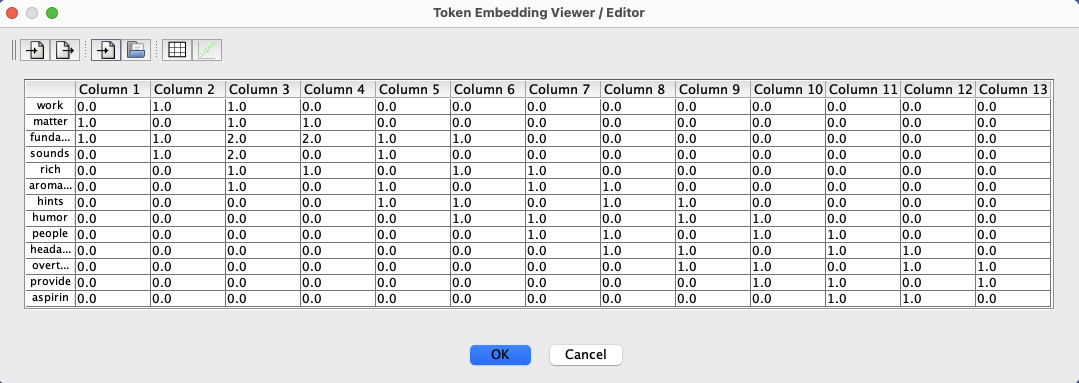
\includegraphics[scale=.5]{./images/full_cooc_matrix.png}
    \caption[Generated using Simbrain.]{Co-occurrence matrix for the example sentences.}
 \label{coocExample}
\end{figure}

After processing the whole document and calculating a co-occurrence matrix, we would use PPMI to weight the vectors. The result can be seen in figure \ref{ppmiExample}.

\begin{figure}[h]
    \centering
    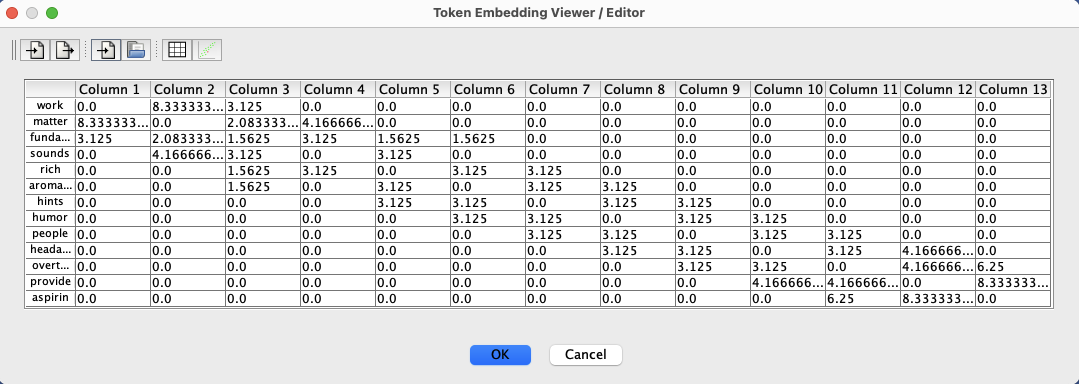
\includegraphics[scale=.45]{./images/weighted_cooc_matrix.png}
    \caption[Generated using SimBrain.]{Resulting co-occurrence matrix after PPMI has been applied.}
 \label{ppmiExample}
\end{figure}


\section{Applications to neural networks}

% Elman: 
% Todo: Elman vs. Chomsky (pull down the Elman commented out stuff here?), maybe Rachel's predictive processing stuff, maybe Bert / GPT 

%These methods mainly track co-occurrence frequencies, which reflect statistical learning theories (SL citations), where learners track label-object co-occurrence statistics. There is also another line of theory in linguistics called predictive processing, where individuals predict future input. This has been used to combat Chomsky's argument about negative evidence (citation), since through disconfirmed predictions, individuals can ``create'' their own negative evidence to learn from (citation for further discussion?). In a similar fashion, neural networks have also been used to generate word embeddings.



